\documentclass[11pt, a4paper]{article}
\usepackage[utf8]{inputenc}
\usepackage{amsmath, amssymb}
\usepackage{graphicx}
\usepackage{hyperref}
\usepackage{xcolor}
\usepackage{listings}
\lstset{
    language=Python,
    basicstyle=\ttfamily\small,
    keywordstyle=\color{blue}\bfseries,
    commentstyle=\color{gray}\itshape,
    stringstyle=\color{orange},
    numberstyle=\tiny\color{gray},
    numbers=left,
    stepnumber=1,
    numbersep=8pt,
    frame=single,
    breaklines=true,
    breakatwhitespace=false,
    showstringspaces=false,
    tabsize=4,
    captionpos=b
}
\usepackage{geometry}
\geometry{margin=1in}

\title{EE 325 Digital Signal Processing \\ Assignment 8: Frequency-Domain Analysis – DTFT and DFS}
\author{PERERA J.D.T. \\ E/21/291}
\date{\today}

\begin{document}
\maketitle

\section{1. DTFT of a Finite-Duration Signal}
The signal is a rectangular pulse of length $N$:
$$ x[n] = \begin{cases} 1 & 0 \le n \le N-1 \\ 0 & \text{otherwise} \end{cases} $$

\subsection{(a) Closed Form Derivation}
The DTFT is defined as:
$$ X(e^{j\omega}) = \sum_{n=-\infty}^{\infty} x[n]e^{-j\omega n} = \sum_{n=0}^{N-1} e^{-j\omega n} $$
This is a geometric series with ratio $r = e^{-j\omega}$ and first term $a=1$:
$$ X(e^{j\omega}) = \frac{1 - (e^{-j\omega})^N}{1 - e^{-j\omega}} = \frac{1 - e^{-j\omega N}}{1 - e^{-j\omega}} $$

\subsection{(b) Form involving sine functions and zero locations}
To express in terms of sine, we pull out half-angle exponential factors:
$$ X(e^{j\omega}) = \frac{e^{-j\omega N/2} (e^{j\omega N/2} - e^{-j\omega N/2})}{e^{-j\omega/2} (e^{j\omega/2} - e^{-j\omega/2})} $$
Using the Euler identity $\sin(\theta) = \frac{e^{j\theta} - e^{-j\theta}}{2j}$:
$$ X(e^{j\omega}) = \frac{e^{-j\omega N/2} \cdot 2j \sin(\omega N/2)}{e^{-j\omega/2} \cdot 2j \sin(\omega/2)} = e^{-j\omega(N-1)/2} \frac{\sin(\omega N/2)}{\sin(\omega/2)} $$

\textbf{Zero Locations:}
Zeros occur when the numerator is zero but the denominator is not.
$$ \sin(\omega N/2) = 0 \Rightarrow \frac{\omega N}{2} = k\pi \Rightarrow \omega = \frac{2\pi k}{N}, \quad k \in \mathbb{Z} $$
Exceptions: When $\sin(\omega/2) = 0$ (i.e., $\omega = 2\pi m$), the value is $N$ (using L'Hopital's rule), so these are not zeros.
Thus, zeros are at $\omega = \frac{2\pi k}{N}$ for $k \ne mN$.

For $N=8$, zeros in $[-\pi, \pi]$ are at:
$$ \omega = \pm \frac{2\pi}{8}, \pm \frac{4\pi}{8}, \pm \frac{6\pi}{8} \Rightarrow \pm \frac{\pi}{4}, \pm \frac{\pi}{2}, \pm \frac{3\pi}{4} $$

\subsection{(c) Main-lobe and Side-lobe Structure}
\begin{itemize}
    \item \textbf{Main Lobe:} Centered at $\omega = 0$. Extends from the first negative zero ($-\frac{2\pi}{N}$) to the first positive zero ($+\frac{2\pi}{N}$).
    \begin{itemize}
        \item Width = $\frac{4\pi}{N}$.
        \item Peak amplitude = $N$ at $\omega = 0$.
    \end{itemize}
    \item \textbf{Side Lobes:} Located between subsequent zeros. The amplitude of side lobes decreases as $\omega$ moves away from 0.
    \begin{itemize}
        \item The width of each side lobe is $\frac{2\pi}{N}$.
    \end{itemize}
\end{itemize}

\section{2. Discrete Fourier Series (DFS)}
Periodic signal with $N=4$:
$$ x[n] = \{1, 2, 3, 4\} \quad \text{for } n=0,1,2,3 $$

\subsection{(a) Compute DFS Coefficients}
The DFS definition is:
$$ \tilde{X}[k] = \sum_{n=0}^{N-1} \tilde{x}[n] e^{-j\frac{2\pi}{N}kn} = \sum_{n=0}^{3} x[n] e^{-j\frac{\pi}{2}kn} $$

\textbf{For k=0:}
$$ X[0] = \sum_{n=0}^{3} x[n] = 1 + 2 + 3 + 4 = 10 $$

\textbf{For k=1:}
$$ X[1] = 1(e^0) + 2(e^{-j\pi/2}) + 3(e^{-j\pi}) + 4(e^{-j3\pi/2}) $$
$$ X[1] = 1 + 2(-j) + 3(-1) + 4(j) = 1 - 3 + j(4-2) = -2 + 2j $$

\textbf{For k=2:}
$$ X[2] = 1(e^0) + 2(e^{-j\pi}) + 3(e^{-j2\pi}) + 4(e^{-j3\pi}) $$
$$ X[2] = 1 + 2(-1) + 3(1) + 4(-1) = 1 - 2 + 3 - 4 = -2 $$

\textbf{For k=3:}
$$ X[3] = 1(e^0) + 2(e^{-j3\pi/2}) + 3(e^{-j3\pi}) + 4(e^{-j9\pi/2}) $$
Note $e^{-j3\pi/2} = j$, $e^{-j3\pi} = -1$, $e^{-j9\pi/2} = e^{-j\pi/2} = -j$.
$$ X[3] = 1(1) + 2(j) + 3(-1) + 4(-j) = 1 - 3 + j(2-4) = -2 - 2j $$

\textbf{Result:}
$$ X[k] = \{10, -2+2j, -2, -2-2j\} $$

\subsection{(b) Real vs Complex and Symmetry}
\begin{itemize}
    \item $X[0]$ and $X[2]$ are real.
    \item $X[1]$ and $X[3]$ are complex.
    \item \textbf{Reason:} For a real-valued sequence $x[n]$, the DFT/DFS is conjugate symmetric:
    $$ X[k] = X^*[N-k] $$
    \begin{itemize}
        \item $X[1] = -2+2j$
        \item $X[4-1] = X[3] = -2-2j$
        \item indeed, $(-2+2j)^* = -2-2j$.
        \item $X[0]$ and $X[N/2]=X[2]$ are their own conjugates, so they must be real.
    \end{itemize}
\end{itemize}

\begin{figure}[h]
    \centering
    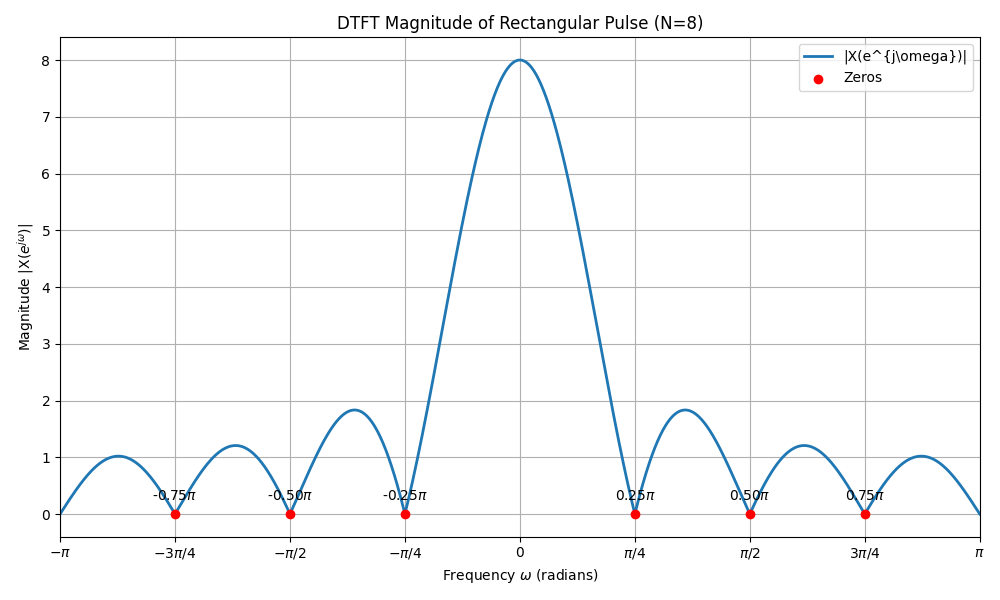
\includegraphics[width=0.8\textwidth]{plots/dtft_magnitude.png}
    \caption{DTFT Magnitude}
    \label{fig:dtft}
\end{figure}

\appendix
\section{Python Source Code}
\textbf{File:} \texttt{assignment8\_dtft.py}
\begin{lstlisting}[caption={DTFT Magnitude of Rectangular Pulse -- Assignment 8}]
import numpy as np
import matplotlib.pyplot as plt
import os

def run_dtft_simulation():
    if not os.path.exists('plots'):
        os.makedirs('plots')

    N = 8
    w = np.linspace(-np.pi, np.pi, 1000)
    num = np.sin(w * N / 2)
    den = np.sin(w / 2)
    X_mag = np.abs(num / den)
    zero_indices = np.where(np.isclose(den, 0))
    X_mag[zero_indices] = N

    plt.figure(figsize=(10, 6))
    plt.plot(w, X_mag, linewidth=2, label='|X(e^{jw})|')
    zeros = [
        -3*np.pi/4, -np.pi/2, -np.pi/4,
        np.pi/4, np.pi/2, 3*np.pi/4
    ]
    plt.scatter(zeros, np.zeros_like(zeros), color='red', zorder=5, label='Zeros')
    for z in zeros:
        plt.annotate(f'{z/np.pi:.2f}pi', (z, 0), xytext=(0, 10),
                     textcoords='offset points', ha='center', fontsize=10)
    plt.title(f'DTFT Magnitude of Rectangular Pulse (N={N})')
    plt.xlabel('Frequency omega (radians)')
    plt.ylabel('Magnitude |X(e^{jw})|')
    plt.xlim([-np.pi, np.pi])
    plt.grid(True)
    plt.legend()
    plt.xticks(
        [-np.pi, -3*np.pi/4, -np.pi/2, -np.pi/4, 0, np.pi/4, np.pi/2, 3*np.pi/4, np.pi],
        ['-pi', '-3pi/4', '-pi/2', '-pi/4', '0', 'pi/4', 'pi/2', '3pi/4', 'pi']
    )
    plt.tight_layout()
    output_path = os.path.join('plots', 'dtft_magnitude.png')
    plt.savefig(output_path)
    print(f"Plot saved to {output_path}")

if __name__ == "__main__":
    run_dtft_simulation()
\end{lstlisting}

\end{document}
